%% Adaptado de 
%% http://www.ctan.org/tex-archive/macros/latex/contrib/IEEEtran/
%% Traduzido para o congresso de IC da USP
%%*****************************************************************************
% Não modificar

\documentclass[twoside,conference,a4paper,12px]{IEEEtran}

%******************************************************************************
% Não modificar
\usepackage{IEEEtsup} % Definições complementares e modificações.
\usepackage[utf8]{inputenc} % Disponibiliza acentos.
\usepackage[english]{babel}
%% Disponibiliza Inglês e Português do Brasil.
\usepackage{latexsym,amsfonts,amssymb} % Disponibiliza fontes adicionais.
\usepackage{theorem} 
\usepackage[cmex10]{amsmath} % Pacote matemático básico 
\usepackage{url} 
\usepackage{bm}
%\usepackage[portuges,brazil,english]{babel}
\usepackage{graphicx}
\usepackage{amsmath}
\usepackage{amssymb}
\usepackage{color}
\usepackage[pagebackref=true,breaklinks=true,colorlinks,bookmarks=false]{hyperref}
\usepackage[tight,footnotesize]{subfigure} 
\usepackage[noadjust]{cite} % Disponibiliza melhorias em citações.

% \usepackage{enumitem}
\usepackage{lscape}
\usepackage{longtable} 
\usepackage[table,xcdraw]{xcolor} % Cores tabelas
% \usepackage{amsthm}
% \usepackage{footnote}
% \usepackage{wasysym}
\usepackage{fancyvrb}
% \usepackage{program}
% \usepackage{algorithm}
% \usepackage{algorithmic}
% \usepackage[noend]{algpseudocode}
\usepackage{multirow}  
\usepackage{epstopdf}
%\usepackage{caption}
% \usepackage{enumitem}
%\usepackage{subcaption}
\usepackage{listings}

\usepackage{color}

\definecolor{codegreen}{rgb}{0,0.6,0}
\definecolor{codegray}{rgb}{0.5,0.5,0.5}
\definecolor{codepurple}{rgb}{0.58,0,0.82}
\definecolor{backcolour}{rgb}{0.95,0.95,0.92}

\lstdefinestyle{mystyle}{
	backgroundcolor=\color{backcolour},   
	commentstyle=\color{codegreen},
	keywordstyle=\color{magenta},
	numberstyle=\tiny\color{codegray},
	stringstyle=\color{codepurple},
	basicstyle=\footnotesize,
	breakatwhitespace=false,         
	breaklines=true,                 
	captionpos=b,                    
	keepspaces=true,                 
	numbers=left,                    
	numbersep=5pt,                  
	showspaces=false,                
	showstringspaces=false,
	showtabs=false,                  
	tabsize=2
}

\lstset{style=mystyle}

\newenvironment{STDdescription}
               {\list{}{\labelwidth 0pt \itemindent-\leftmargin
                        \let\makelabel\descriptionlabel}}
               {\endlist}
% \newcommand*\descriptionlabel[1]{\hspace\labelsep
%                                 \normalfont\bfseries #1}

\DeclareMathOperator*{\argmax}{arg\,max}

%%*****************************************************************************

\begin{document}
%\selectlanguage{brazil}
\renewcommand{\IEEEkeywordsname}{Palavras-chave}
% \renewcommand{\lstlistingname}{Código}

%%*****************************************************************************

\urlstyle{tt}
% Indicar o nome do autor e o curso/nível (grad-mestrado-doutorado-especial)
\title{Redes Artificiais de Arquitetura Variante}
\author{%
\IEEEauthorblockN{	Lucas O. David\,\IEEEauthorrefmark{1}}
 \IEEEauthorblockA{%
                   Ciência da Computação - Pós-Graduação \\
                   E-mail: 	\IEEEauthorrefmark{1}ld492@drexel.edu}
}

\maketitle

%%*****************************************************************************
% Resumo do trabalho
\begin{abstract}
%  O resumo deve conter uma breve descrição sobre várias partes do seu trabalho que serão tratadas no decorrer do texto. 
%  Primeiramente, pode-se descrever brevemente o problema no qual você está trabalhando: 
%  Por que você está desenvolvendo este trabalho? Qual a motivação para este desenvolvimento? 
%  Por que ele é importante? O resumo deve conter também um breve descritivo da metodologia que você usou no desenvolvimento: 
%  Que problema foi tratado? Como a solução foi construída/desenvolvida? Quais as tecnologias utilizadas? 
%  Finalmente, deve falar um pouco sobre os resultados que você conseguiu: o resultado final ficou bom? 
%  Quais os seus principais diferenciais? Qual a eficiência do desenvolvimento?

apesar do grande desenvolvimento de redes neurais artificiais aplicadas a problemas cada vez mais complexos, pouco foi feito no que diz respeito à otimização da arquitetura dos modelos utilizados. Este trabalho propoe que esta otimização ocorra pela busca sobre o espaço de arquiteturas possíveis, percorrendo-o de forma a alcançar um candidato à solução que seja tanto eficaz na generalização do conjunto de dados em mãos quando enxuto em relação ao seu número de parâmetros, caracterizando assim um problema de busca clássico. Resultados empíricos preliminares sugerem que tal busca resulta em refinamentos interessantes das arquiteturas de redes.

\end{abstract}

% Indique três palavras-chave que descrevem o trabalho
\begin{IEEEkeywords}
  Aprendizado de Máquina, Redes Neurais Artificiais.
\end{IEEEkeywords}

%%*****************************************************************************
% Modifique as seções de acordo com o seu projeto

\section{Introdução}

% Na introdução você deve descrever os aspectos mais relevantes sobre a revisão bibliográfica que fez e do problema que você decidiu tratar. 
% Quais foram os pontos estudados/pesquisados? Quais os outros trabalhos similares ao seu que você encontrou? 
% Também na introdução espera-se que você descreva um pouco sobre a motivação de trabalhar com esse tema. 
% A descrição do seu trabalho será feita em detalhes nas próximas seções do artigo.
% No final da introdução, é comum inserir um parágrafo descrevendo o que será encontrado em cada seção no restante do seu texto. 
% Exemplo: Este trabalho encontra-se organizado da seguinte forma: a seção 2 apresenta X. A seção 3 descreve Y. 
% Os resultados são apresentados na seção 4, e as conclusões são apresentadas na seção 5.

Redes neurais artificiais têm recorrentemente apresentado efetivas soluções para problemas de aprendizado de máquina. Elas podem ser, entretanto, computacionalmente custosas. Com um alto número de parâmetros causado por uma quantidade significativa de camadas e unidades, tais redes exigem alto desempenho computacional, \textit{hardware} específico (e.g. GPUs) e longos períodos de trainamento. Na última decada, também é notável uma aumento do emprego de redes convolucionais em problemas de tratamento e interpretação de sinais (e.g. audio, video, texto), característicamente profundas e compostas por um número massivo de parâmetros.

Um problema imediato ao decidir se utilizar de redes neurais artificiais é encontrar uma arquitetura adequada ao problema em questão. Devido a grande dificuldade deste problema, muitos autores recorrem à reutilização de arquiteturas já existentes, que tiveram seu bom comportamento demonstrado por experimentos empíricos em domínios de problema similares.

Contrariamente à escolha de arquiteturas tradicionais, é possível buscar uma arquitetura através da exploração do espaço de escolhas possíveis, preferindo por aquelas que adequadamente abordam o problema, enquanto minimizando sua complexidade. Como o número de arquiteturas é possívelmente infinito, percorrer o espaço eficientemente é de fundamental importância.

Este trabalho tem como principal objetivo a modelação do problema de otimização de arquitetura como um problema de busca, podendo ser portanto resolvido por simples agentes inteligentes baseados em utilidade e algoritmos de busca clássicos (e.g. \textit{Hill-Climbing} e algoritmos genéticos).

O restante deste relatório está organizado da seguinte forma: na Seção~\ref{sec:conceitos} são apresentados conceitos importantes no entendimento do trabalho; o trabalho proposto, bem como o modelo utilizado para a tarefa são descritos na Seção~\ref{sec:trabalhoproposto}. Resultados de experimentos são discutidos na Seção~\ref{sec:resultados}. Finalmente, as considerações finais são feitas na Seção~\ref{sec:consideracoes_finais}.

%******************************************************************************
%******************************************************************************
\section{Conceitos Fundamentais}
\label{sec:conceitos}
%******************************************************************************
%******************************************************************************

Nesta sessão, conceitos chave para o entendimento do trabalho proposto serão brevemente enunciados. Tais conceitos vão desde uma breve descrição das representações numéricas de redes neurais artificias ao conceito de busca

\subsection{Redes Neurais Artificiais}

Uma rede neural artificial é um modelo de aprendizado de máquina inspirado na estrutura de uma rede neural biológica \cite{yegnanarayana2009artificial}. Associada à uma arquitetura específica, uma rede neural se utiliza de seus parâmetros para transformar um sinal de entrada em outro. Por exemplo, um sinal de entrada pode ser transformado em um de menor dimensionalidade (redução dimensional); gerar probabilidades de pertencimento à múltiplicas classes (classificação); ou regredir um ou mais valores contínuos (regressão). Fig. \ref{fig:nn_base} exemplifica abstratamente uma rede neural, composta por três camadas com $1$, $N$ e $3$ unidades, respectivamente.

\begin{figure}[!ht]
\centering
	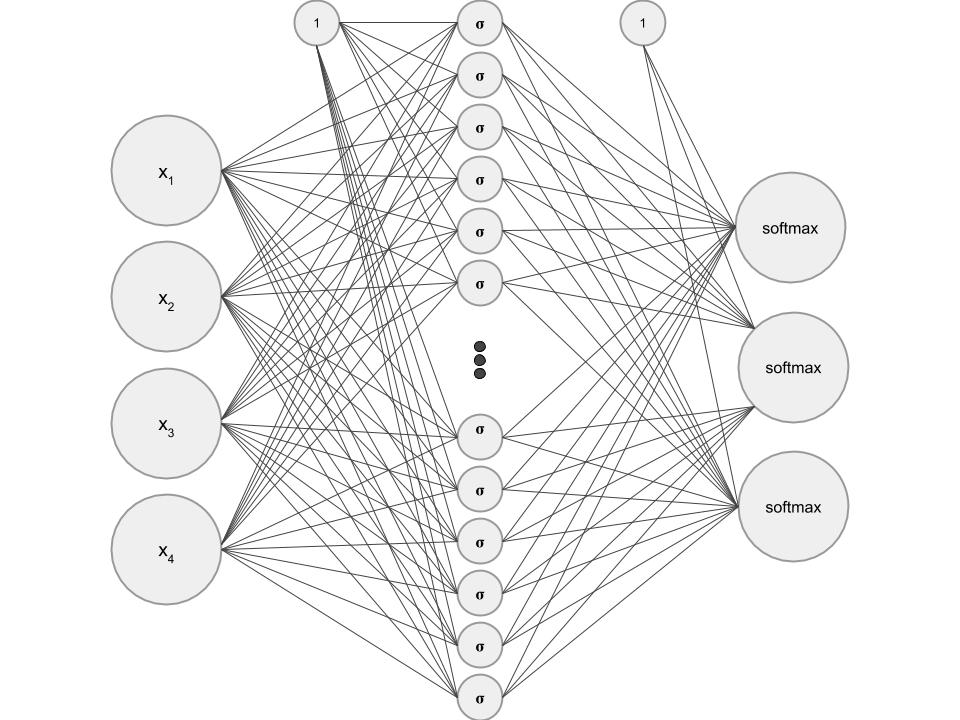
\includegraphics[width=.48\textwidth]{assets/nn-base}
	\caption{Ilustração de uma rede neural com três camadas, com função de ativação $\sigma$ na segunda camada e $softmax$ como função de ativação na terceira.}
	\label{fig:nn_base}
\end{figure}

Uma rede neural também pode ser definida algebricamente, onde sua saída é um $y$ em função do sinal de entrada e de seus parâmetros $\theta$.

\subsubsection{Redes Densas}

também conhecidas como \textit{Multilayer Perceptron} (MLPs), são redes caracterizadas pela total conexão de todos os neurônios da camada $i$ para os da camada $i -1$ e os da camada $i + 1$. A propagação do sinal (i.e. a saída da rede $\bm y$) pode ser representada na seguinte forma algébrica:
\newline\newline
Seja $\bm X \in \mathbb{R}^{n \times f}$ um conjunto de $n$ amostras descritas por $f$ atributos, $\theta = (\bm{W, b})$ os parâmetros da rede e $\sigma$ uma função denominada ``ativação". Então,

$$\bm{y(X) = \sigma(W \cdot X + b})$$

\subsubsection{Redes Convolucionais}

baseadas especificamente no cortex visual, essas redes propagam o sinal através da operação de convolução entre o sinal de entrada e \textit{kernels} (descritores basicos de padrões), sendo ideais para identificar padrões locais \cite{krizhevsky2012imagenet}. Ademais, a sucessiva concatenação de convoluções, eventualmente intercaladas por camadas de \textit{pooling} (ou sub-amostragem), é capaz de construír efetivos reconhecedores para padrões complexos, como objetos e faces.

Uma camada convolucional de uma rede convolucional pode ser descrita pela seguinte equação:

\begin{align*}
	(\bold I \ast \bold K)(i, j) &= \sum_{k=0}^h \sum_{l=0}^w \bold I (i - k, j -l)\bold K(k, l)\\
	y_{i,j} &= \bold I \ast \bold K(i, j)
\end{align*}

Ou seja, a própria convolução discreta; limitada inferiormente e superiormente; e definida sobre tensores de rank 2 (matrizes).

\begin{figure}[!ht]
	\centering
	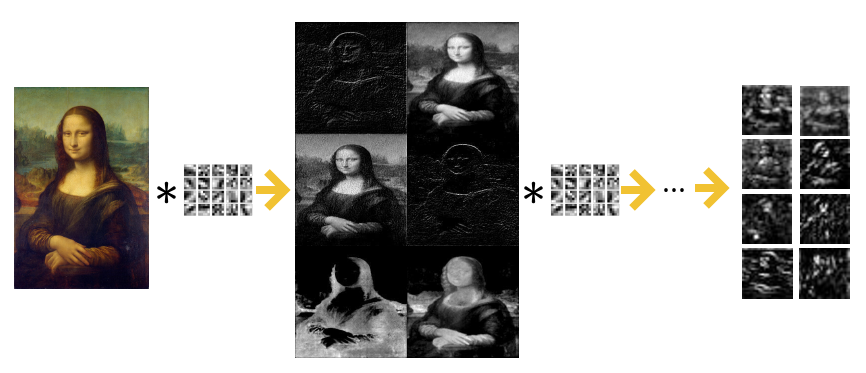
\includegraphics[width=.48\textwidth]{assets/cn-base}
	\caption{Ilustração de um sinal de entrada (uma pintura) sendo propagado por uma rede convolucional -- a arquitetura VGG19 \cite{simonyan2014very}, treinada sobre o conjunto de dados ImageNet \cite{ILSVRC15}.}
	\label{fig:cn_base}
\end{figure}

Finalmente, é importante destacar a utilizando de redes dense concatenadas à convolucionais, criando efetivos modelos de classificação/regressão sobre amostras representadas sinais de alta dimensionalidade (e.g. imagens, sons, texto) \cite{krizhevsky2012imagenet, simonyan2014very}.

\subsection{Intelligência Artificial Clássica}

\subsubsection{Mundo}

a modelação de um problema computacionalmente descritível. Por exemplo, o caso de estudo clássico da \textbf{limpeza de um ambiente} sujos pelo agente de limpeza automatizado \cite{russell2003artificial}.

\subsubsection{Estado}

um objeto representativo de condições possíveis para o mundo. Por exemplo, o vetor $(1, 1, 1, 1, 0)$ pode representar uma condição do problema de \textbf{limpeza de ambiente} onde os quatro primeiros elementos representam se um ambiente está ou não sujo, enquanto o último sinaliza a posição corrente do agente.

\subsubsection{Agente}

uma entidade inserida no mundo, que o percebe com \textbf{sensores} e atua sobre ele através de \textbf{atuadores} \cite{russell2003artificial}. Dentre os inúmeros tipos de agentes, destaca-se o agente \textbf{baseado em utilidade}, que associa a cada estado um valor real e, caso seja um agente racional, buscará estados que maximizem esse valor.

\subsubsection{Espaço de busca}

um grafo direcionado que indica como os estados do mundo se relacionam.

\subsubsection{Busca}

A atividade de navegar pelo espaço de possíveis estados de um mundo a fim de se encontrar um estado objetivo ou o caminho para ele. Fig. \ref{fig:ex_search} exemplifica a \textbf{busca em largura} sobre um espaço qualquer.

\begin{figure}[!ht]
	\centering
	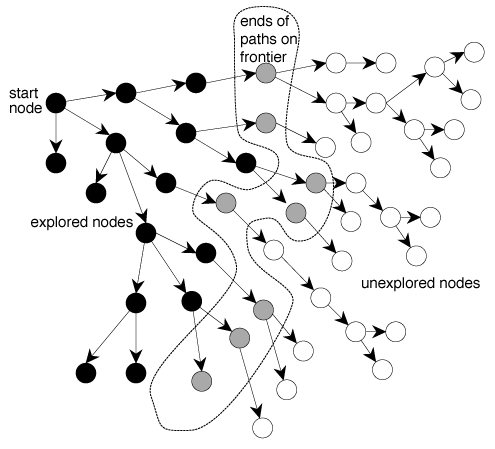
\includegraphics[width=.3\textwidth]{assets/ex_search}
	\caption{Ilustração da execução de uma \textbf{busca em largura}, em um espaço de busca para um problema qualquer.}
	\label{fig:ex_search}
\end{figure}

Dentre as diversas buscas existentes, destacamos duas:

\paragraph{\textit{Hill-Climbing} (exemplo de busca)}

um tipo de busca local onde estamos preocupados em percorrer o espaço de forma a maximizar a utilidade do estado atual para o agente. A Fig. \ref{fig:search-hill-climbing} exemplifica essa busca em um espaço contínuo, de uma única variável.

\begin{figure}[!ht]
	\centering
	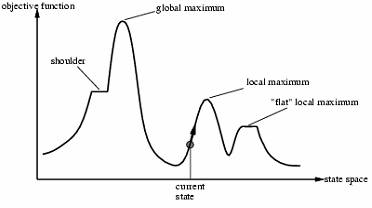
\includegraphics[width=.3\textwidth]{assets/search-hill-climbing}
	\caption{\textit{Hill-Climbing} sobre um espaço contínuo.}
	\label{fig:search-hill-climbing}
\end{figure}

Naturalmente, \textit{Hill-Climbing} não garante o obtenção de máximo global. Entretanto, uma forma simples de fortificar as respostas seria reiniciar a busca multiplas vezes a partir de um ponto aleatório (uma estratégia conhecida como \textit{random-restart}).

\paragraph{Algoritmos Genéticos (exemplo de busca)}

um modelo de busca inspirado na teoria de seleção natural de Darwin \cite{darwin1909origin}. Aqui, uma população de estados é iterativamente submetida a operadores de criação (e.g. \textit{cross-over}, mutação) e seleção de tal forma a reforçar positivamente a sobrevivência dos estados com alto valor de utilidade. A tabela \ref{tbl:ga} exibe o operador de \textit{cross-over} com um único ponto de corte (gene 2) sobre dois indivíduos A e B, resultando em dois novos indivíduos (C e D).

\begin{table}[!ht]
	\normalsize
	\renewcommand\tabcolsep{4.5pt}
	\renewcommand{\arraystretch}{1.2}
	\centering
	\begin{tabular}{|l|cc|cccc|}
		\hline  
		indivíduo A & 0 & 0 & 1 & 1 & 0 & 1 \\\hline
		indivíduo B & 1 & 1 & 0 & 1 & 0 & 0 \\\hline\hline
		indivíduo C & 0 & 0 & 0 & 1 & 0 & 0 \\\hline
		indivíduo D & 1 & 1 & 1 & 1 & 0 & 1 \\\hline		
	\end{tabular}
	\caption{A operação de \textit{cross-over} entre dois indivíduos (A e B).}
	\label{tbl:ga}
\end{table}


%******************************************************************************
%******************************************************************************
\section{Trabalho Proposto}
\label{sec:trabalhoproposto}
% Nesta seção descreva de forma abrangente, porém clara e organizada, o seu trabalho.

Nesta seção, será apresentado uma abordagem para o problema de seleção de arquiteturas.

\subsection{Definição do problema}

Seja $(\bm{X, y})$ um conjunto de dados pré-determinado, o mundo é definido como o problema de encontrar a arquitetura de rede neural capaz de generalizar adequadamente o conjunto $(\bm{X, y})$, ao passo que possui o menor número de parâmetros possíveis (e.g. camadas e unidades nas camadas).

\subsection{Arquiteturas representadas por estados do mundo}

Define-se uma representação que descreva possíveis arquiteturas para as redes. Tal representação se constitui por duas coleções de elementos, onde cada coleção contém camadas descritas por pares (\# unidades/kernels, função de ativação), como exemplificado pela listagem \ref{lst:arch}.

\begin{lstlisting}[language=Python, caption={Representação de uma arquitetura de rede neural artificial como um estado no espaço de busca.}, label={lst:arch}]
S = {
  'dense': ((4096, 'relu'), (10, 'softmax'))
  'conv': ((32, 'relu'), (128, 'relu'))
}
\end{lstlisting}

\subsection{Transições entre arquiteturas}

O agente alcança novas arquiteturas ao aplicar os operadores descritos abaixo à uma ou mais arquiteturas já existentes. Da lista, os três primeiros são necessárias à busca utilizando algoritmos genéticos, enquanto as demais são essenciais à buscas locais, como o \textit{Hill-climbing}.

\begin{enumerate}
	\item \textbf{Random:} produz um arquitetura aleatória.
	\item \textbf{Cross-over:} combina duas arquiteturas, resultando em uma terceira.
	\item \textbf{Mutate:} produz uma mudança de intensidade $q$ com probabilidade $p$ em cada camada existente.
	\item \textbf{Reduce conv:} reduz o número de camadas convolucionais.
	\item \textbf{Reduce dense:} reduz o número de camadas densas.
	\item \textbf{Reduce kernels:} reduz para $\frac{2}{3}$ o número de \textit{kernels} na última camada convolucional.
	\item \textbf{Reduce units:} reduz para $\frac{2}{3}$ o número de unidades na última camada densa.
	\item \textbf{Increase conv:} aumenta o número de camadas convolucionais.
	\item \textbf{Increase dense:} aumenta o número de camadas densas.
	\item \textbf{Increase kernels:} aumenta para $\frac{3}{2}$ o número de \textit{kernels} na última camada convolucional.
	\item \textbf{Increase units:} aumenta para $\frac{3}{2}$ o número de unidades na última camada densa.
\end{enumerate}

\subsection{Utilidade}

A fim de direcionar a busca à resultados satisfatórios, é necessário a definição de uma função de utilidade que beneficie ``boas" arquiteturas e prejudique arquiteturas ``ruins". Esta função de utilidade $u$ é definida da seguinte forma:

\begin{align*}
	u(S) &= -h(S)\\
	h(S) &= \lambda_1 \sum_{i=1}^{|\text{layers}|} \frac{\text{units}_i - \text{min-units}}{\text{max-units} - \text{min-units}}\\
	&+ \lambda_2 \frac{\text{layers} - \text{min-layers}}{\text{max-layers} - \text{min-layers}}\\
	&+ \lambda_3 \text{train-loss}\\
	&+ \lambda_4 \text{validation-loss}
\end{align*}

Onde $\lambda_1 .. \lambda_4$ são constantes definidas pelo usuário, ponderando a importância de cada métrica para a função de custo $h$.

A utilidade de uma arquitetura pode ser interpretada da seguinte forma: uma arquitetura (estado) terá mais alta utilidade quando apresentar mais baixo número de unidades e \textit{kernels}, mais baixo número de camadas e mais baixas perdas de treino e validação.


\section{Resultados e Discussão}
\label{sec:resultados}

A busca por arquiteturas foi experimentada em dois conjuntos diferentes. Nesta seção, serão descritos os resultados de tais experimentos.

\subsection{Conjunto de dados \textbf{Digits}}

Contendo imagens em escala cinza de 10 diferentes dígitos, \textbf{Digits} tem como tarefa associada a correta classificação de uma amostra em 10 classes distintas.

Utilizando uma população de 50 arquiteturas, com probabilidade de mutação $p = .25$ e fator de mutação $q = .5$ e mantendo o processo evolutivo por 5 gerações, obteve-se uma arquitetura (listagem \ref{lst:digits_ga}) com um maior número de camadas densas, porém com considerável redução em perda de treino (de 11.78 para 7.4) e validação (de 3.84 para 2.2).

\begin{lstlisting}[language=Python, caption={Resultado da busca por algoritmo genético sobre o conjunto \textbf{Digits}.}, label={lst:digits_ga}]
# Initial architecture candidate:
architecture {
  'conv': [(47, 'relu')],
  'dense': [(10, 'softmax')]
]}:
|-train-loss: 11.782062
|-validation loss: 3.841851

...
# Final architecture candidate:
architecture {
  'conv': [(47, 'relu')],
  'dense': [(40, 'relu'), (10, 'softmax')]
]}:
|-train-loss: 7.403219
|-validation loss: 2.209876
\end{lstlisting}

\subsection{Conjunto de dados \textbf{Cifar-10}}

\textbf{Cifar-10} contém imagens em formato RGB percentendes à 10 distintas classes relacionadas à elementos do mundo real (e.g. aviões, carros, cavalos, navios).

Aqui, \textit{Hill-Climbing} foi utilizado para partir de uma arquitetura com maior número de camadas convolucionais e alcançar uma arquitetura de notável menor complexidade (\ref{lst:cifar_hc}), enquanto mantendo ambas perdas de treinamento e teste similares às originais.

\begin{lstlisting}[language=Python, caption={Resultado da busca por \textit{Hill-Climbing} sobre o conjunto de dados \textbf{Cifar-10}.}, label={lst:cifar_hc}]
# Initial architecture candidate:
architecture {
  'conv': [(47, 'relu'), (47, 'relu'),
           (54, 'relu'), (104, 'relu'),
           (200, 'relu')],
  'dense': [(75, 'relu'), (10, 'softmax')]
}:
|-train-loss: 0.429305
|-validation loss: 2.174616

...
# Final architecture candidate:
architecture {
  'conv': [(39, 'relu'), (127, 'relu'),
           (136, 'relu')],
  'dense': [(79, 'relu'), (10, 'softmax')]
]}:
|-train-loss: 0.422453
|-validation loss: 2.145460
\end{lstlisting}


%******************************************************************************
%******************************************************************************
\section{Considerações finais}
\label{sec:consideracoes_finais}

% Nesta seção, faça uma análise geral de seu trabalho, levando em conta todo o processo de desenvolvimento e os resultados. 
% Quais os seus pontos fortes? Quais os seus pontos fracos? Quais aspectos de sua metodologia de trabalho foram positivas? Quais foram negativas? 
% O que você recomendaria (ou não recomendaria) a outras pessoas que estejam realizando trabalhos similares aos seus? 
Este trabalho apresentou uma possível modelagem do problema de seleção de arquiteturas como um problema de inteligência artificial clássico, resolvível por agentes baseados em utilidade e algoritmos de buscas dos mais variados. O modelo foi testado em dois conjuntos de dados distintos, exibindo interessantes resultados em ambos.

Como trabalhos futuros, destaca-se a necessidade de acelerar o processo de busca em si através do melhoramento do desempenho da avaliação de utilidade de uma determinada arquitetura. Este processo requer, atualmente, o treinamento completo dos modelos (iniciados com pesos aleatórios) descritos por cada arquitetura. Uma opção a se considerar é experimentar com a transferência parcial de pesos, possívelmente acelerando a convergência do treino e, portanto, das avaliações.

%******************************************************************************
%******************************************************************************
% Referências - Definidas no arquivo mybib.bib

\bibliographystyle{IEEEtran}
\bibliography{references}

%******************************************************************************
\end{document}
